\section{Results}
\subsection{results of single models}
Before merging the three models together it must be controlled whether each model is implemented correctly for itself. The pictures of the models simulation results are the guide for this. Sometimes there are discrepanies between the puplished model and the picture which should represent the model.  Hereafter, the implementation process for each of the models is described.\\
To better retrace the implementation steps it is recommended to read the paper for the hog \cite{Zi_2010}, ion \cite{Gerber_2016} and volume model  \cite{volumeModel}.

\subsubsection{Ion model}
The challanges with the implementation of the ion model were, that the presented equations, initial values and parameters did not result in the intended system behaviour. \\
After an in-depth analysis of the equation there were two anomalies:

\begin{enumerate}
	\item the calculation of the change of the inner proton ion concentration has \emph{Bf} as an undefined parameter
	\item the fluxes have the wrong units
\end{enumerate}

For solving the problem with the undefined parameter in (1) the ODE was constructed by deriving the formula for the calculation of the pH value for diluted solution \ref{pHforDilution}
\begin{equation*}
	pH = - log_{10}([H^+])\\
\end{equation*}
\begin{equation}\label{pHforDilution}
	\frac{d}{dt}pH = \frac{d}{dt}(-log_{10}([H^+])) = - \frac{1}{ln(10)} \frac{d}{dt}ln([H^+]) = - \frac{1}{ln(10)}\frac{1}{H^+} \frac{dH^+}{dt}
\end{equation}
and combine it with the equation \ref{pHchange} for the change of the pH Value as a result of proton flux (\cite{martinafroehlich})
\begin{equation}\label{pHchange}
	\frac{d}{dt}pH_{in} = \frac{J_H \cdot Surface}{V_{in} \cdot pbc}
\end{equation}
	
The equation \ref{usedProtonFlux} 
\begin{equation}\label{usedProtonFlux}
- \frac{1}{ln(10)} \frac{1}{H^+}\frac{dH^+}{dt} = \frac{J_H \cdot Surface}{V_{in} \cdot pbc}\\
\Rightarrow \frac{dH^+}{dt}=-\frac{J_H \cdot Surface \cdot ln(10) \cdot H^+}{V_{in} \cdot pbc}
\end{equation}

was used for modelling the change of the inner proton concentration.\\\\
To solve the problem with the wrong units it was identified, that the equation for the reported fluxes only missed the unit Kelvin $K$ in its numerator. Multiplying the equation with the temperature $T$ solved this problem and resulted in the equation \ref{IonFlux}.
\begin{figure}[htbp]
	
	\begin{minipage}{0,5\textwidth}
		
		\includegraphics[width=\textwidth]{picture/Ion_Paper.png}
		
		\label{IonPaper} 
	\end{minipage}
	\begin{minipage}{0,5\textwidth}
		
		\includegraphics[width=\textwidth]{picture/ion_examine.png}
		
		\label{IonImplemented} 
	\end{minipage}
	\caption{left: membrane voltage in the ion paper for different NaCl stimulus (0.01 mM - 10 mM); right: the simulated implemented ion model for the same stimulus range }
\end{figure}


\subsection{hog model}
For the implemtation of the hog model, the \textit{Table S1-S3} and the Matlab code for the used $NaCl$ impulse in \textit{Code S1 } in the supporting informations of the paper were implemented in the python3 environment. No difficulties were encountered. 

\begin{figure}[htbp]
	
	\begin{minipage}{0,5\textwidth}
		
		\includegraphics[width=\textwidth]{picture/Hog_Paper.png}
		
		\label{hogPaper} 
	\end{minipage}
	\begin{minipage}{0,5\textwidth}
		
		\includegraphics[width=\textwidth]{picture/hog_examine.png}
		
		\label{hogImplemented} 
	\end{minipage}
	\caption{}
\end{figure}

\subsection{volume model}
The volume model could not be implemented with only the corresponding paper because the model wants to describes the change in the non-osmolytic volume $V_b$ but missed to note down an equation for this.\\
After consultation with my supervisior and one of the author of the model about this information gap, it was recommended that I use the already implemented volume model in their local network "YCM" as a template. After translating this template in my own software structure, no problems were encountered. In the appendix I documented the used ODE, algebraic equation, parameter and initial values for this model. 
% schritte der volume model implementierung
\begin{figure}[htbp]
	
	\begin{minipage}{0,5\textwidth}
		
		\includegraphics[width=\textwidth]{picture/Volume_Paper.png}
		
		\label{volumePaper} 
	\end{minipage}
	\begin{minipage}{0,5\textwidth}
		
		\includegraphics[width=\textwidth]{picture/volume_examine.png}
		
		\label{volumeImplemented} 
	\end{minipage}
	\caption{}
\end{figure}


\subsection{merging of the models}
The process of merging models is a tricky task. There exists some good guideline \cite{Liebermeister2008ValidityAC} for this.
Hereafter, the used essential steps are sketched:
\begin{enumerate}
	\item equations: One of the first steps in the process of model merging is to control whether there is a conflict between assumptions of the description of the biological systems. Conflicts must be resolved by combining equation terms or discard some informations
	\item names: Find all the overlaps in the variable and parameter naming and convert them to a common sets of names
	\item units: Standardize all used units for the parameter and initial values to a common set. In this process new factors where give to individual values if the unit changes requires that.
\end{enumerate}
Changes in the equation design (ODE and algebraic equation) were done in the process of merging the models and are presented below:
\begin{table} [h]
	\footnotesize
\begin{center} 
	\caption{changes in the equation design}
\begin{tabular} {l l l l l l l l}
%&  \multicolumn{2}{c}{changing equation}  \\ \hline
& changes & reason\\
internal / external osmolyt concentration & $c = \sum ([Ionen]+[other osmolyte])$ & simplification\\ 
internal / external presure & $\pi = c \cdot R \cdot T	$ & simplification\\
ion x changes & $\frac{J_x \cdot CellSurface}{CellVolume} \cdot 10^{6}$ & unit harmonization\\
sorbitol stimulus & $\frac{d}{dt}[Sorbitol]=0$ & implementation of sorbitol stimulus with the assumation that sorbitol can not diffuse over the plasma membrane; in ODE format because due to the simulation design this approach results in less memory data\\
uptake / dilution of osmotically active compounds & removed & replaced with the equation for the ion and glycerol
\end{tabular}
\label{changesOnTheModels}
\end{center}
\end{table}

In the whole process of merging we must consider their biochemical interpretation to maintain the plausblity of the model \cite{Liebermeister2008ValidityAC}. No parameter value was changed in its biological interpretation.\\\\
Initial values were changed because, as we can see in figure \ref{IntersectionsOfTheModels}

\begin{figure}[h!]
	\begin{center}
		\begin{minipage}{0,8\textwidth}
			
			\includegraphics[width=\textwidth]{picture/model_intersections.png}
			\caption{Response of Hog1PPn} 
			\label{IntersectionsOfTheModels} 
		\end{minipage}
	\end{center}
\end{figure}

 multiple components are used in several models. These components have different quantities in the initial assumptions. One of the main difference was the assumption of the cell volume $V_{cell}$ in the hog model ($V_{cell}=58fL $) and the volume model ($V_{cell} \approx 0.27fL$). To solve this problem we simulated the volume model until $V_{cell}$ also has the value of $58fL$. We assumed the ODE values at this time point as the initial values for the corresponding substance in the merged model. \\\\
We removed the volume related variables and $\pi_t$ from the hog model because the calculation of $\pi_t$ in the volume model was based on updated insights.


%%% bis hier hin eigentlich ganz ok
\subsection{combined model}
For the analysis and validation of the merged model we choosed the nuclear phophorylated Hog1 (Hog1PPn) as the control substance. Hog1PPn is also used in the hog model as the output because it regulates the expression of hundred of genes \cite{Zi_2010}. We borrowed the idea of a drug response curve from the theme field pharmocokinetic (zitieren: hier das Buch!!!) as a visualized output showed below.  \\
(hier noch das falsche Bild, da Simulation noch nicht ganz fertig)
\begin{figure}[h!]
	\begin{center}
		\begin{minipage}{0,8\textwidth}
			
			\includegraphics[width=\textwidth]{picture/model_intersections.png}
			\caption{Response of Hog1PPn} 
			\label{DrugResponseCurve} 
		\end{minipage}
	\end{center}
\end{figure}

\subsubsection{single models with the initial values from the combined model}
After implement the initial values from the combined model back to the single models, no difference for the hog model was simulated. The reason for this lays in the simple reason, that we only changed the initial values from the ion and the volume model in the combined model.\\
The problem for compering the simulation results for the volume model is the fact, that the original data from the Github-Account of the ...

\newpage
